\documentclass[a4paper,11pt]{article}
\usepackage[utf8]{inputenc}
\usepackage[german]{babel}
\usepackage{geometry}
\usepackage{graphicx}
\usepackage{parskip}
\usepackage{titlesec}
\usepackage{hyperref}

\setcounter{secnumdepth}{4}

\titleformat{\paragraph}
{\normalfont\normalsize\bfseries}{\theparagraph}{1em}{}
\titlespacing*{\paragraph}
{0pt}{3.25ex plus 1ex minus .2ex}{1.5ex plus .2ex}


\geometry{a4paper, margin=2.5cm}
\graphicspath{{images/}}

\begin{document}

\begin{table}[h]
		\centering
		\footnotesize
		\begin{tabular}{| p{1.5cm} | p{2.5cm} | p{2cm} | p{2cm} | p{2cm} |}
			\hline
			                           & Verantwortliche Teammitglieder (Organisation, Anlegen der Dokumentenversion, Moderation, Abgabe)                                   & Anwesende während der Meetings                                                                                                     & (Online-) Beiträge zum Inhalt durch                                                                                                & Korrektur-gelesen durch                                                                                                            \\
			\hline
			Dokument Sprint Version 1 & Paul Schröder, Eric Buthmann, Yanik Buthmann, Mathis Behrendt, Adrian Gode, Niklas Krüger, Kevin Zellmer & Paul Schröder, Eric Buthmann, Yanik Buthmann, Mathis Behrendt, Adrian Gode, Niklas Krüger, Kevin Zellmer & Paul Schröder, Eric Buthmann, Yanik Buthmann, Mathis Behrendt, Adrian Gode, Niklas Krüger, Kevin Zellmer & Paul Schröder, Eric Buthmann, Yanik Buthmann, Mathis Behrendt, Adrian Gode, Niklas Krüger, Kevin Zellmer \\
			\hline
		\end{tabular}
	\end{table}


\section{Sprint Planung}

Wir haben insgesamt vier Sprints, dementsprechend teilen wir die Umsetzung unserer User Stories in vier Sprints auf und testen die Funktionalität unserer Software immer am Ende eines Sprints. Dementsprechend haben wir pro Sprint 6 User Stories die in Tasks umgewandelt werden und vom Team umgesetzt werden müssen. Im ersten Sprint haben wir den Fokus auf das Herstellen einer Grundfunktionalität unserer Software, wie zum Beispiel das Erstellen eines Accounts, das Einloggen in einen erstellten Account und weitere Grundfunktionen. Grundlegend soll die Umsetzung der ausgewählten sechs User Stories dazu führen, dass wir eine Basis haben für unsere Software, auf der wir aufbauen und dann die komplexeren User Stories befriedigen können und unser Programm somit Schritt für Schritt in der Komplexität zu erweitern.

Die Auswahl der User Story S1.1 wurde getroffen, da das Anlegen eines Accounts essentiell dafür ist, um sich später einloggen zu können, Backlogs zu erstellen et cetera, es legt also den Grundstein für die Funktionalität. Die User Story S1.2 ist wichtig, um dann mit dem angelegten Account auch arbeiten zu können, denn ohne Einloggen Funktion ist ein Account nicht von Nutzen. Die User Story S1.3 ist wichtig, da das Zurücksetzen eines Passwortes ebenfalls eine essenzielle Funktion ist, um das Programm überhaupt nutzen zu können, da bei Vergessen des Passworts beispielsweise das Programm nicht mehr nutzbar ist, da man sich nicht mehr einloggen kann. Die User Story S4.1 wurde gewählt, da das Erstellen eines Backlogs, der Kern unseres Programms ist und auf dieser Funktion bauen dann die folgenden Sprints und deren User Stories auf. User Story S5.1 haben wir gewählt, da es nahe liegt beim Erstellen der Funktionalität zum Anlegen eines Accounts auch die Funktionalität zum Einrichten des dazugehörigen Profils bereitzustellen. Als letzte User Story in diesem Sprint haben wir S3.1 also das Hinzufügen von User Stories in ein Backlog, das ist ebenfalls eine Kernaufgabe und wird ebenfalls der Grundstein sein für spätere Spezifikationen.

Wir sind folgendermaßen vorgegangen, um die User Stories in Tasks aufzuteilen. Wir haben eine User Story betrachtet und haben diese in eine sinnvolle Reihenfolge gebracht, damit zuerst die User Story zum Anlegen eines Accounts bearbeitet wird und dann die zum Zurücksetzen eines Passworts beispielsweise. Anschließend haben wird analysiert, was in jeder einzelnen Schicht unserer Schichtenarchitektur geschehen muss, damit das Programm diese Funktionalität der User Story bereitstellen kann. Das heißt was muss im Data-Layer geschehen (im ersten Sprint größtenteils DB-Tabellen initialisieren), dann was im Service Layer geschehen muss (Endpunkte etablieren) und im Presentation/Application Layer (Frontend erstellen, erstmal Plain HTML). Dementsprechend haben wir dann die Tasks formuliert. Wir haben die Tasks für unsere User Stories so angeordnet, dass die Reihenfolge auch die Abhängigkeit darstellt, das heißt die Tasks, die weiter unten angeordnet sind, sind abhängig von der erfolgreichen Bearbeitung der oberen Tasks.

Unser Team besteht aus sieben Teammitgliedern, deshalb haben wir unser Team in zwei Zweiergruppen und in eine Dreiergruppe geteilt und dann jeweils zwei User Stories pro Team abgearbeitet. So konnten wir effizient arbeiten, da es direkte Kommunikationswege gab und keine Schwierigkeiten durch zu viele Personen oder verschiedenen Ansätzen, auch um zeitlich möglichst effizient arbeiten zu können.

\vspace{1em}
\noindent\textit{Hinweis: Das vollständige Sprintbacklog ist unter \href{run:./Sprintbacklog.pdf}{Sprintbacklog.pdf}, sowie \href{https://git.informatik.uni-rostock.de/softwaretechnik-ws-2025-26/uebung3/team3/projekt-team3-uebung3/-/blob/main/abgabedokumente/Sprintbacklog.pdf?ref_type=heads}{im Gitlab} zu finden.}

\section{Verfeinerte Architektur}

\subsection{Task/User Stories}
\subsubsection{Modellierung für User Story S1.1: Account anlegen}
\paragraph{Modellierung verfeinerter Struktur}

Die geplanten Tasks für diese User Story sind befinden sich im Sprintbacklog. 

Im Application Layer befindet sich das \texttt{RegistrationForm}, das die Nutzereingaben entgegennimmt und Erfolg oder Fehler anzeigt. Im Presentation Layer liegt der \texttt{UserController}, der über \texttt{POST /register} die Daten an die Fachlogik weitergibt. Die eigentliche Registrierungslogik liegt im \texttt{RegistrationService}, unterstützt durch \texttt{Validator}, \texttt{PasswordHasher} und \texttt{AccountRepository}. Im Data Layer greift das Repository auf die Tabelle \texttt{accounts} zu.

Die Klasse \texttt{RegistrationForm} enthält die Felder \texttt{username}, \texttt{email}, \texttt{password} und \texttt{confirmPassword}. Der \texttt{UserController} nimmt Registrierungsanfragen entgegen und gibt Erfolgs- oder Fehlerantworten zurück. Der \texttt{RegistrationService} prüft Eingaben, kontrolliert auf bereits existierende Accounts, ruft das Passwort-Hashing auf und speichert neue Accounts. Der \texttt{Validator} prüft Pflichtfelder, Email-Format und Passwortübereinstimmung. Der \texttt{PasswordHasher} sorgt dafür, dass Passwörter nicht im Klartext gespeichert werden. Das \texttt{AccountRepository} übernimmt den Datenbankzugriff.

Diese Aufteilung unterstützt \textbf{Separation of Concerns} und ist erweiterbar für spätere User Stories. Als Design Patterns kommen das \textbf{Repository Pattern} (\texttt{AccountRepository}) und das \textbf{Service Pattern} (\texttt{RegistrationService}) zum Einsatz.
\newpage
\begin{figure}[h]
    \centering
    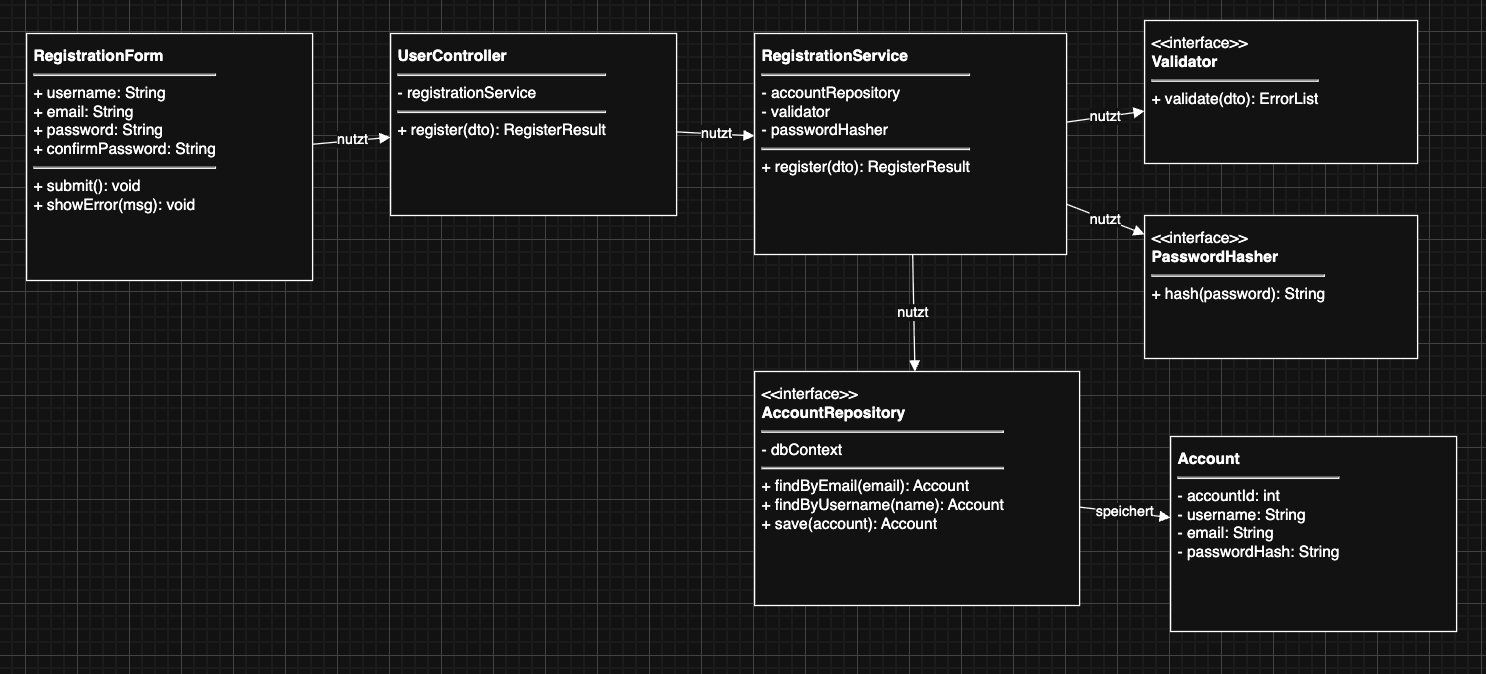
\includegraphics[width=\textwidth]{2_1_story1.png}
    \caption{Verfeinerte Struktur für User Story S1.1: Account anlegen}
\end{figure}

\paragraph{Modellierung verfeinerter Interfaces und Datenstrukturen}

Für die Kommunikation zwischen den Komponenten werden zwei zentrale Datenstrukturen verwendet: \texttt{RegisterDTO} und \texttt{RegisterResult}.

Das \texttt{RegisterDTO} enthält die Felder \texttt{username}, \texttt{email}, \texttt{password} und \texttt{confirmPassword}. Es wird vom \texttt{RegistrationForm} an den \texttt{UserController} übergeben und bildet die Eingabedaten der Registrierung ab. Das \texttt{RegisterResult} enthält ein \texttt{success}-Flag, eine \texttt{message} und eine Liste von \texttt{errors}. Es dient als einheitliche Rückgabe von Controller an Formular.

Die Interfaces zwischen den Komponenten sind wie folgt verfeinert: Der \texttt{UserController} stellt die Methode \texttt{register(dto: RegisterDTO): RegisterResult} bereit, die die Anfrage über \texttt{POST /register} entgegennimmt und an den Service delegiert. Der \texttt{RegistrationService} bietet ebenfalls eine Methode \texttt{register(dto: RegisterDTO): RegisterResult}, die Validierung, Duplikatsprüfung, Hashing und Speicherung durchführt. Der \texttt{Validator} stellt \texttt{validate(dto: RegisterDTO): List<String>} bereit, um Pflichtfelder, Email-Format und Passwortübereinstimmung zu prüfen. Der \texttt{PasswordHasher} bietet \texttt{hash(password: String): String} zum Erzeugen eines sicheren Hashs. Das \texttt{AccountRepository} verfügt über \texttt{findByUsername(username: String): Account?} und \texttt{findByEmail(email: String): Account?} für die Duplikatsprüfung sowie \texttt{save(account: Account): void} zum Speichern eines neuen Accounts.

Gespeichert wird die Datenstruktur \texttt{Account} in der Tabelle \texttt{accounts}. Sie enthält \texttt{id} (eindeutig), \texttt{username} (eindeutig), \texttt{email} (eindeutig) und \texttt{password\_hash}. Das Passwort wird ausschliesslich als Hash gespeichert. Benutzername und Email müssen eindeutig sein, um doppelte Accounts zu verhindern.

\texttt{RegisterDTO} ist bewusst von \texttt{Account} getrennt, weil das Feld \texttt{confirmPassword} nur für die Validierung benötigt und nicht persistiert wird. \texttt{RegisterResult} ermöglicht eine einheitliche Fehler- und Erfolgskommunikation zwischen Controller und Frontend. Die Methoden des \texttt{AccountRepository} sind gezielt auf die Anforderungen der Registrierung zugeschnitten: Duplikatsprüfung per \texttt{findBy}-Methoden und Persistierung per \texttt{save}.
\newpage
\begin{figure}[h]
    \centering
    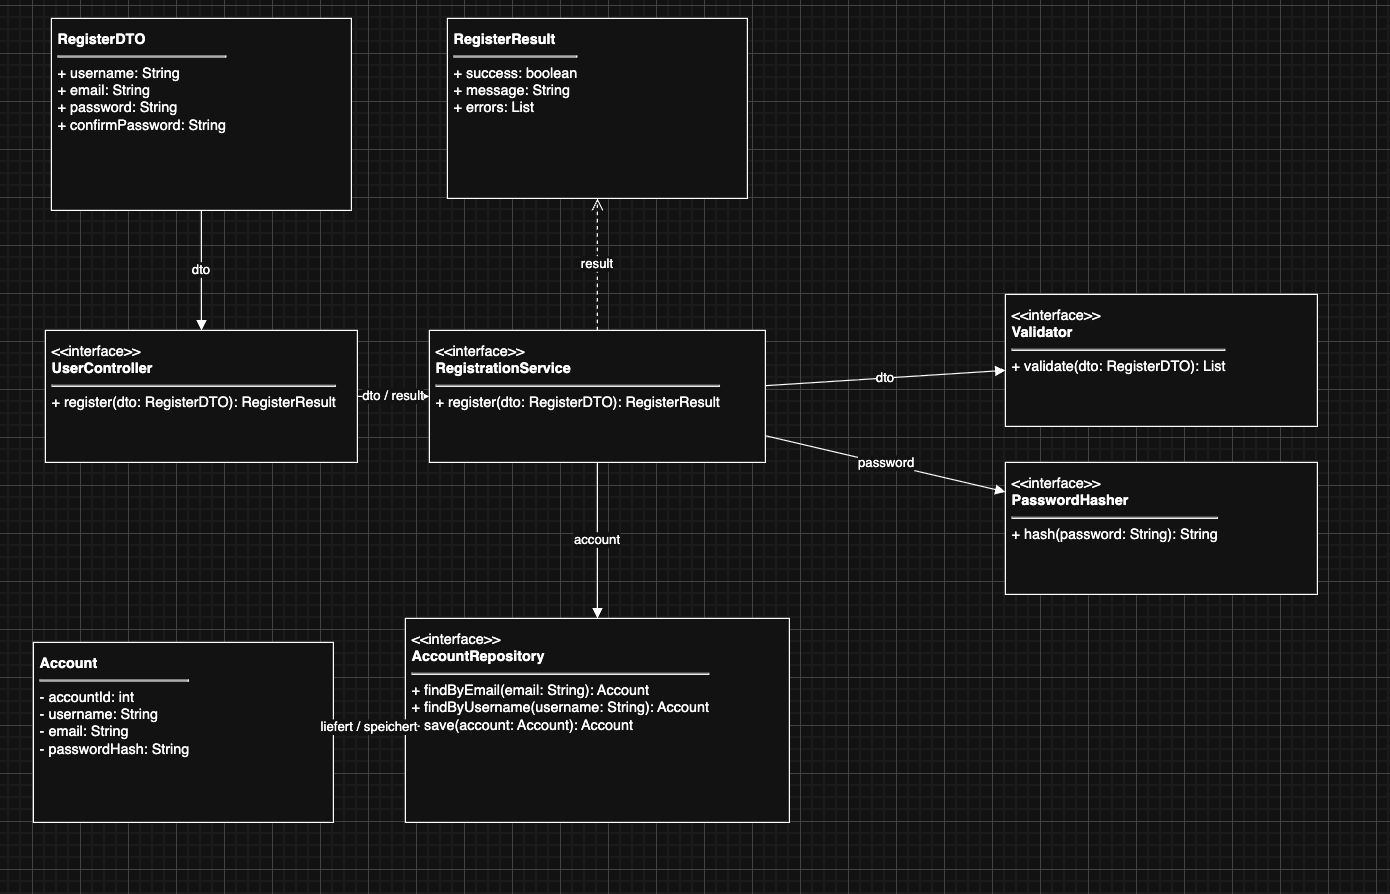
\includegraphics[width=\textwidth]{2_2_story1.png}
    \caption{Verfeinerte Interfaces und Datenstrukturen für User Story S1.1: Account anlegen}
\end{figure}

\paragraph{Modellierung relevanter Verhaltensaspekte}

Das Verhalten der Registrierung wird durch ein Sequenzdiagramm modelliert, das die Kommunikation über die definierten Interfaces zeigt. Der Ablauf ist: Das \texttt{RegistrationForm} sendet ein \texttt{RegisterDTO} an den \texttt{UserController}, dieser ruft \texttt{RegistrationService.register(dto)} auf. Der Service delegiert an \texttt{Validator.validate(dto)}. Bei Fehlern wird sofort ein \texttt{RegisterResult} mit Fehlerstatus zurückgegeben. Bei gültigem Input ruft der Service \texttt{AccountRepository.findByUsername()} und \texttt{findByEmail()} auf. Existiert bereits ein Account, folgt eine Fehlerantwort. Andernfalls wird \texttt{PasswordHasher.hash(password)} aufgerufen, ein \texttt{Account}-Objekt erzeugt und per \texttt{AccountRepository.save(account)} gespeichert. Der Controller gibt das \texttt{RegisterResult} an das Formular zurück.

Auf weitere Verhaltensdiagramme wie State Machines oder Aktivitätsdiagramme wird verzichtet, da der Registrierungsablauf linear ist, nur einen Akteur betrifft und keine komplexen Zustandswechsel enthält. Das Sequenzdiagramm genügt, um die Komponentenkommunikation und die beiden Alternativpfade (ungültige Eingaben, bestehender Account) vollständig darzustellen.

\begin{figure}[h]
    \centering
    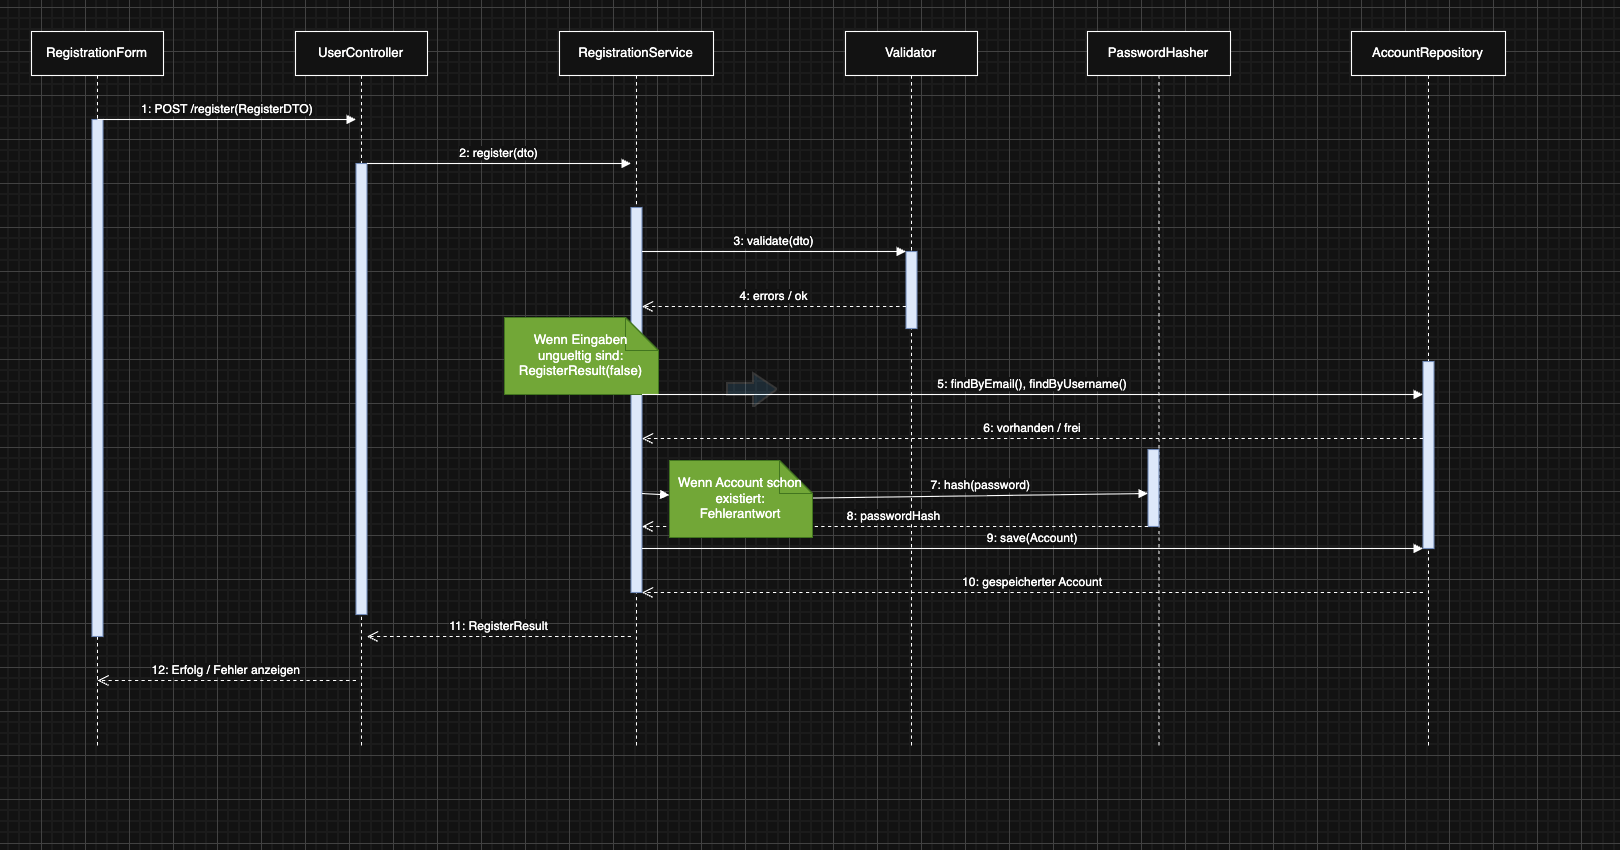
\includegraphics[width=\textwidth]{2_3_story1.png}
    \caption{Sequenzdiagramm für User Story S1.1: Account anlegen}
\end{figure}

\newpage

\subsubsection{Modellierung für User Story S1.2: Einloggen}

\paragraph{Modellierung verfeinerter Struktur}

Für den Login wird die bestehende 4-Schichten-Architektur um folgende Klassen erweitert: Im Application Layer nimmt das \texttt{LoginForm} (Felder: \texttt{usernameOrEmail}, \texttt{password}) die Nutzereingaben entgegen. Im Presentation Layer delegiert der \texttt{UserController} über \texttt{POST /login} an den \texttt{LoginService} im Service Layer, der die zentrale Fachlogik enthält: Eingabeprüfung, Accountsuche, Passwort-Hash-Vergleich und Session-Erstellung. Unterstützt wird er durch den \texttt{PasswordHasher} (hier für den Vergleich, nicht für die Erzeugung), den \texttt{SessionManager} (Sitzungsverwaltung) und das \texttt{AccountRepository} (Datenbankzugriff auf Tabelle \texttt{accounts}) im Data Layer.

Die Komponenten \texttt{PasswordHasher} und \texttt{AccountRepository} werden aus User Story S1.1 wiederverwendet, was die Erweiterbarkeit der Architektur bestätigt. Neu hinzu kommen \texttt{LoginService} und \texttt{SessionManager}. Diese Aufteilung unterstützt \textbf{Separation of Concerns}, da Oberfläche, Fachlogik, Session-Verwaltung und Datenzugriff klar getrennt bleiben. Als Design Patterns kommen das \textbf{Repository Pattern} (\texttt{AccountRepository}) und das \textbf{Service Pattern} (\texttt{LoginService}) zum Einsatz -- konsistent zur Registrierung und erweiterbar für spätere User Stories wie Passwort zurücksetzen.

\paragraph{Modellierung verfeinerter Interfaces und Datenstrukturen}

Für den Login werden drei Datenstrukturen zwischen den Komponenten ausgetauscht: \texttt{LoginDTO} (Felder: \texttt{usernameOrEmail}, \texttt{password}), \texttt{LoginResult} (Felder: \texttt{success}, \texttt{message}, \texttt{redirectUrl}) und \texttt{Session} (Felder: \texttt{sessionId}, \texttt{accountId}). Das \texttt{LoginDTO} bildet die Eingabedaten ab, das \texttt{LoginResult} dient als einheitliche Rückgabe für Erfolg und Fehler, und die \texttt{Session} repräsentiert die aktive Sitzung nach erfolgreichem Login.

Die verfeinerten Interfaces sind: Der \texttt{UserController} stellt \texttt{login(dto: LoginDTO): LoginResult} bereit und delegiert an den \texttt{LoginService}, der ebenfalls \texttt{login(dto: LoginDTO): LoginResult} anbietet. Der \texttt{PasswordHasher} stellt \texttt{verify(password: String, hash: String): boolean} für den Vergleich bereit. Der \texttt{SessionManager} bietet \texttt{create(accountId: String): Session} zur Sitzungserstellung. Das \texttt{AccountRepository} stellt \texttt{findByUsernameOrEmail(input: String): Account?} für die Accountsuche bereit.

Gespeichert werden zwei Datenstrukturen: Die \texttt{Account}-Daten liegen in der Tabelle \texttt{accounts} (aus S1.1 bekannt). Zusätzlich wird die \texttt{Session} serverseitig persistiert, damit der Nutzer nach dem Login identifiziert bleibt und auf seine Daten zugreifen kann.

\texttt{LoginDTO} ist von \texttt{Account} getrennt, da nur minimale Eingabedaten benötigt werden. \texttt{LoginResult} ermöglicht eine einheitliche Kommunikation inkl. Weiterleitung. Die \texttt{Session} als eigene Datenstruktur ist notwendig, weil die Sitzungsverwaltung unabhängig von der Account-Logik bleiben soll -- das unterstützt Separation of Concerns und erleichtert spätere Erweiterungen wie Logout oder Session-Timeout.

\paragraph{Modellierung relevanter Verhaltensaspekte}

Das Verhalten des Logins wird durch ein Sequenzdiagramm modelliert. Der Ablauf über die Interfaces ist: Das \texttt{LoginForm} sendet ein \texttt{LoginDTO} an \texttt{UserController.login(dto)}. Dieser delegiert an \texttt{LoginService.login(dto)}, der zunächst \texttt{AccountRepository.findByUsernameOrEmail(input)} aufruft. Wird kein Account gefunden, wird ein \texttt{LoginResult} mit Fehlerstatus zurückgegeben. Andernfalls ruft der Service \texttt{PasswordHasher.verify(password, hash)} auf. Bei fehlgeschlagenem Vergleich folgt ebenfalls eine Fehlerantwort. Bei Erfolg wird \texttt{SessionManager.create(accountId)} aufgerufen und ein \texttt{LoginResult} mit Weiterleitung zurückgegeben.

Auf State Machines oder Aktivitätsdiagramme wird verzichtet, da der Login-Ablauf linear ist, nur einen Akteur betrifft und lediglich zwei Alternativpfade (Account nicht gefunden, Passwort falsch) aufweist. Das Sequenzdiagramm genügt, um die Komponentenkommunikation über die Interfaces vollständig darzustellen.
\subsubsection{Modellierung für User Story S1.3}



\paragraph{Modellierung verfeinerter Struktur}

Das Zurücksetzten des Pasworts wird durch die bestehende 4-Schichten-Architektur sowie einigen weiteren Klassen realisiert. Im Application Layer nimmt \texttt{ResetForm} die Eingabe des Nutzers entgegen(Felder: UsernameorEmail). Im Presentation Layer wird über den \texttt{UserController} und dem POST-Endpunkt /reset-password die Anfrage an den \texttt{PasswordResetService} im Service Layer gesendet. Hier wird die Prüfung ob ein entsprechender Account existiert geprüft und dann ein temporäres \texttt{ResetToken} zum Zurücksetzten erzeugt. Unterstützung erfolgt durch das \texttt{AccountRepository} sowie den \texttt{TokenGenerator} und dem \texttt{PasswordHasher} zur Sicheren Speicherung des neuen passworts. Der Datenbankzugriff des \texttt{AccountRepository} erfolgt im Data Layer.


\paragraph{Modellierung verfeinerter Interfaces und Datenstrukturen}

Die Darstellung der Struktur von Userstory S1.3 wird durch Folgendes Klassendiagramm Modelliert. Desweiteren Werden folgende Datenstrukturen Grundlegend verwendet: \texttt{requestpasswordreset}, \texttt{ResetToken}, \texttt{resetPassword} sowie ResetResult. \texttt{requestpasswordreset} enthält die Eingabe des Nutzers, also die E-Mail oder den Benutzernamen. \texttt{ResetToken} enthält die Informationen über das Token, wie die ID, den zugehörigen Account, den Token-Wert und das Ablaufdatum. \texttt{resetPassword} enthält die Informationen für das Zurücksetzen des Passworts, also den Token und das neue Passwort. \texttt{ResetResult} enthält Informationen über den Erfolg oder Fehler der Operation.

\begin{figure}[h]
    \centering
    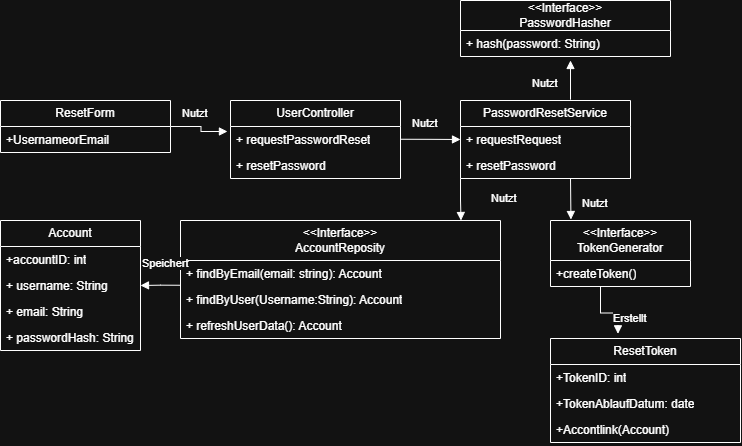
\includegraphics[width=\textwidth]{Klassendiagramm213.png}
    \caption{Klassendiagramm für User Story S1.3: Passwort zurücksetzen}
\end{figure}


\paragraph{Modellierung relevanter Verhaltensaspekte}

Die Darstellung des Verhaltens der User Story S1.3 wird durch ein Sequenzdiagramm Modelliert. Der Ablauf ist wie folgt: Das \texttt{ResetForm} sendet ein \texttt{requestpasswordreset} an den \texttt{UserController}, dieser delegiert dann an den \texttt{PasswordResetService}. Dieser prüft über das \texttt{AccountRepository}, ob ein Account mit der angegebenen E-Mail oder dem Benutzernamen existiert. Wenn kein Account gefunden wird, wird ein \texttt{ResetResult} mit Fehlerstatus zurückgegeben. Andernfalls generiert der Service ein \texttt{ResetToken} über den \texttt{TokenGenerator} und speichert es im Repository. Bei validierten Token, wird das Passwort mittels \texttt{PasswordHasher} gehasht und aktualisiert den Account über das Repository. Abschließend wird ein \texttt{ResetResult} mit Erfolg oder Fehler zurückgegeben.

\begin{figure}[h]
    \centering
    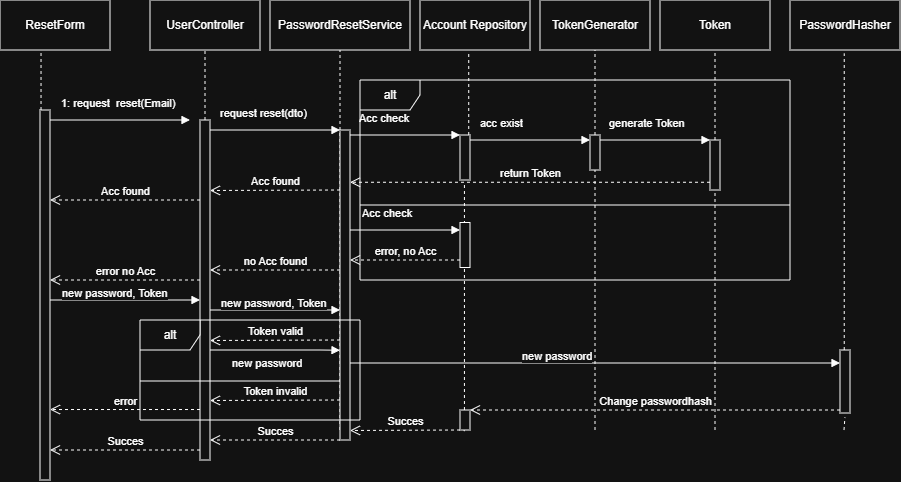
\includegraphics[width=\textwidth]{Sequenzdiagramm213.png}
    \caption{Sequenzdiagramm für User Story S1.3: Passwort zurücksetzen}
\end{figure}

\newpage
\subsubsection{Modellierung für User Story S3.1}
\paragraph{Modellierung verfeinerter Struktur}
Das Anlegen einer Task erfolgt ähnlich zum erstellen eines Backlogs. Hierbei muss jedoch neben Namen und ID der Task auch ein entsprechendes Backlog, das durch das Attribut bl\_id gegeben ist, in dem die Task erstellt werden soll, identifiziert werden. TaskCreation (Application Layer) übergibt die Daten der zu erstellenden Task an den TaskController (Presentation Layer). Dieser übergibt dieselben Daten weiter an TaskService (Service Layer). TaskService leitet die Daten dann anschließend weiter an das Task Repository(Data Layer) und sendet anschließend eine Rückmeldung an TaskCreation. Das Repository verwaltet den Datenbankzugriff und speichert die Task. Zusätzlich kann das Repository Tasks nach Namen und nach ID suchen.
Diese Aufteilung unterstützt Seperation of Concerns und verwendet Repository Pattern sowie Service Pattern.

\paragraph{Modellierung verfeinerter Interfaces und Datenstrukturen}
Zugriffe erfolgen nur über Interfaces. Andere Erweiterungen sind nicht nötig, da das Anlegen eines Backlogs unkomplex ist.
\begin{figure}[h]
    \centering
    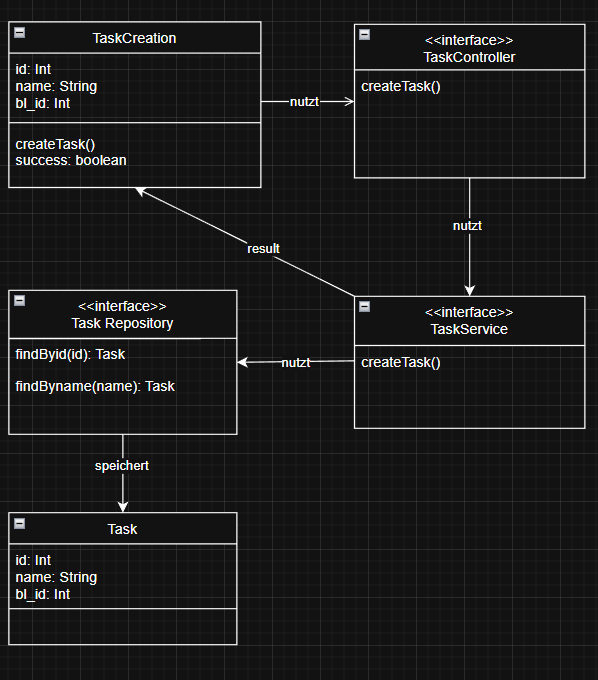
\includegraphics[width=10cm]{diagram31.png}
    \caption{Klassendiagramm für User Story S3.1: Task erstellen}
\end{figure}

\paragraph{Modellierung relevanter Verhaltensaspekte}
Das erstellen einer Task wird hier anschaulich in einem Sequenzdiagramm dargestellt. Dieses entspricht ganz dem Ablauf, der in 2.1.4.1 beschrieben wurde.
\begin{figure}[h]
    \centering
    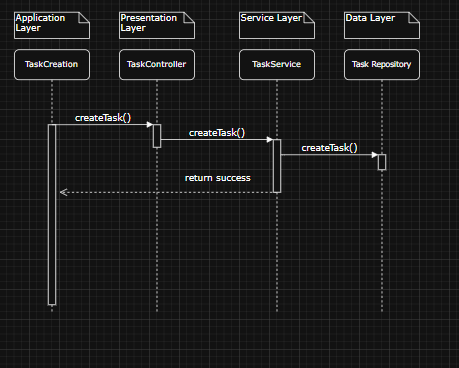
\includegraphics[width=10cm]{diagram32.png}
    \caption{Sequenzdiagramm für User Story S3.1: Task erstellen}
\end{figure}
\newpage
\subsubsection{Modellierung für User Story S4.1}
\paragraph{Modellierung verfeinerter Struktur}
BacklogCreation findet im Application Layer statt. Dort kann mit Angabe eines Namen und einer ID die Erstellung eines Backlogs initiiert werden. Diese Daten werden dann weitergereicht zum BacklogController (Presentation Layer) und anschließend zum BacklogService (Service Layer). Der BacklogService sendet die Daten an das BacklogRepository und sendet anschließend eine Rückmeldung an BacklogCreation. Das BacklogRepository ist für den Zugriff auf die Datenbank verantwortlich (Data Layer). Zusätzlich kann das Repository Backlogs nach Namen oder nach der ID suchen.
Diese Aufteilung unterstützt Seperation of Concerns und verwendet Repository Pattern sowie Service Pattern.

\paragraph{Modellierung verfeinerter Interfaces und Datenstrukturen}
Zugriffe erfolgen nur ueber Interfaces. Andere Erweiterungen sind nicht nötig, da das Anlegen eines Backlogs unkomplex ist.
\begin{figure}[h]
    \centering
    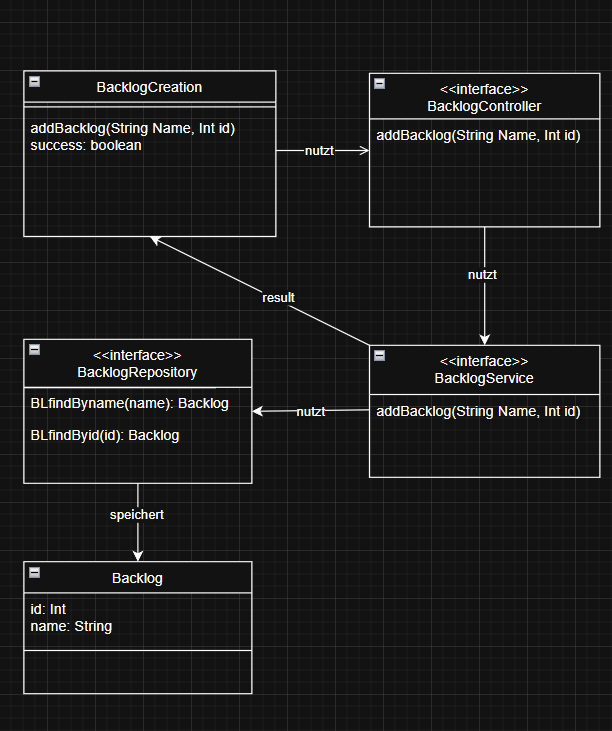
\includegraphics[width=10cm]{diagram41.png}
    \caption{Klassendiagramm für User Story S4.1: Backlog erstellen}
\end{figure}
\newpage
\paragraph{Modellierung relevanter Verhaltensaspekte}
Der Ablauf des Anlegens eines Backlogs wird durch ein Sequenzdiagramm modelliert. Der Ablauf entspricht der Beschreibung aus 2.1.5.1.
\newpage
\begin{figure}[h]
    \centering
    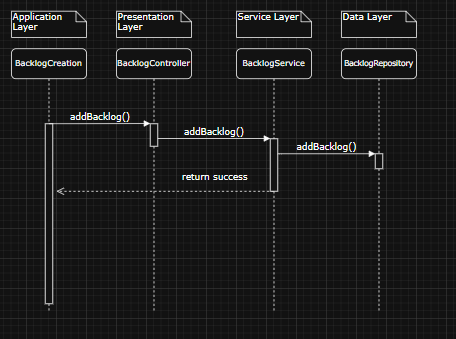
\includegraphics[width=10cm]{diagram42.png}
    \caption{Sequenzdiagramm für User Story S4.1: Backlog erstellen}
\end{figure}
\subsubsection{Modellierung für User Story S5.1}
\paragraph{Modellierung verfeinerter Struktur}
\paragraph{Modellierung verfeinerter Interfaces und Datenstrukturen}
\paragraph{Modellierung relevanter Verhaltensaspekte}

\newpage
\subsection{Tracing}

Die folgende Tabelle zeigt, welche User Stories durch welche Klassen umgesetzt werden.

\begin{table}[h]
\centering
\small
\renewcommand{\arraystretch}{1.4}
\begin{tabular}{| p{3.5cm} | p{10cm} |}
\hline
\textbf{User Story} & \textbf{Wichtigste Klassen} \\
\hline
\textbf{S1.1} - Account anlegen &
\texttt{RegistrationForm}, \texttt{UserController}, \texttt{RegistrationService}, \texttt{Validator}, \texttt{PasswordHasher}, \texttt{AccountRepository}, \texttt{Account} \\
\hline
\textbf{S1.2} - Einloggen &
\texttt{LoginForm}, \texttt{UserController}, \texttt{LoginService}, \texttt{PasswordHasher}, \texttt{SessionManager}, \texttt{AccountRepository}, \texttt{Session} \\
\hline
\textbf{S1.3} - Passwort zurücksetzen &
\texttt{ResetForm}, \texttt{UserController}, \texttt{PasswordResetService}, \texttt{TokenGenerator}, \texttt{AccountRepository}, \texttt{ResetToken} \\
\hline
\textbf{S3.1} - Task erstellen &
\texttt{TaskCreation}, \texttt{TaskController}, \texttt{TaskService}, \texttt{TaskRepository}, \texttt{Task} \\
\hline
\textbf{S4.1} - Backlog erstellen &
\texttt{BacklogCreation}, \texttt{BacklogController}, \texttt{BacklogService}, \texttt{BacklogRepository}, \texttt{Backlog} \\
\hline
\textbf{S5.1} - Nutzerprofil &
\texttt{ProfileForm}, \texttt{ProfileController}, \texttt{ProfileService}, \texttt{ProfileRepository}, \texttt{UserProfile} \\
\hline
\end{tabular}
\caption{Tracing: User Stories zu modellierten Klassen}
\end{table}

\bigskip

\noindent\textbf{Beschreibung der Beziehungen:}

\textbf{S1.1 - Account anlegen:} Das \texttt{RegistrationForm} nimmt die Eingaben des Nutzers entgegen und gibt sie an den \texttt{UserController} weiter. Der \texttt{RegistrationService} prüft die Eingaben mit dem \texttt{Validator}, stellt sicher dass der Account noch nicht existiert (via \texttt{AccountRepository}) und hasht das Passwort mit dem \texttt{PasswordHasher}, bevor der neue \texttt{Account} gespeichert wird.

\textbf{S1.2 - Einloggen:} Das \texttt{LoginForm} gibt die Zugangsdaten an den \texttt{UserController} weiter, der den \texttt{LoginService} aufruft. Dieser sucht den Account im \texttt{AccountRepository} und prüft das Passwort über den \texttt{PasswordHasher}. Bei Erfolg erstellt der \texttt{SessionManager} eine neue \texttt{Session}. \texttt{AccountRepository} und \texttt{PasswordHasher} werden aus S1.1 wiederverwendet.

\textbf{S1.3 - Passwort zurücksetzen:} Das \texttt{ResetForm} gibt die E-Mail des Nutzers weiter. Der \texttt{PasswordResetService} generiert einen Reset-Token (gespeichert als \texttt{ResetToken}) und aktualisiert nach Eingabe eines neuen Passworts den Account über das \texttt{AccountRepository}. Auch hier werden \texttt{AccountRepository} und \texttt{PasswordHasher} aus S1.1 wiederverwendet.

\textbf{S3.1 - Task erstellen:} \texttt{TaskCreation} übergibt die Eingaben an den \texttt{TaskController}, der sie zum \texttt{TaskService} weiterleitet. Dieser speichert die neue \texttt{Task} über das \texttt{TaskRepository} in der Datenbank.

\textbf{S4.1 - Backlog erstellen:} \texttt{BacklogCreation} gibt Name und ID an den \texttt{BacklogController} weiter, der den \texttt{BacklogService} aufruft. Dieser legt ein neues \texttt{Backlog}-Objekt an und speichert es über das \texttt{BacklogRepository}.

\textbf{S5.1 - Nutzerprofil:} Das \texttt{ProfileForm} zeigt persönliche Daten an und nimmt Änderungen entgegen. Der \texttt{ProfileController} leitet diese an den \texttt{ProfileService} weiter, der die Daten über das \texttt{ProfileRepository} speichert oder abruft. \texttt{UserProfile} referenziert dabei den zugehörigen \texttt{Account} aus S1.1.

\end{document}





